\documentclass[letterpaper,12pt]{article}

\usepackage{tabularx} % extra features for tabular environment
\usepackage{amsmath}  % improve math presentation
\usepackage{graphicx} % takes care of graphic including machinery
\usepackage[margin=1in,letterpaper]{geometry} % decreases margins
\usepackage[final]{hyperref} % adds hyper links inside the generated pdf file
\usepackage{ctex}
\usepackage{titlesec}
%\usepackage{CJKutf8, CJK}
\usepackage{makecell}                 % 三线表-竖线
\usepackage{booktabs}                 % 三线表-短细横线
% \usepackage{natbib}
\usepackage{graphicx}				  % 表格单元格逆时针
\usepackage{multirow}				  % 合并单元格
\usepackage{array}
\usepackage{amssymb}				  % 勾
\usepackage{amsmath}
\usepackage{longtable}                % 导入 longtable 宏包,表格自动换行
\usepackage{caption}
\usepackage{subcaption}               % 设置子图
\usepackage{color}					  % 文本颜色包
\usepackage{xcolor}
\usepackage{bbm}					  % 输入指示函数
\usepackage{tablefootnote}			  % 表格注释
\usepackage{pythonhighlight}

\usepackage{listings}                 % 导入代码块
\usepackage{xcolor}
\lstset{
	numbers=left, 
	tabsize=1,
	columns=flexible, 
	numberstyle=  \small, 
	keywordstyle= \color{ blue!70},
	commentstyle= \color{red!50!green!50!blue!50}, 
	frame=shadowbox, % 阴影效果
	rulesepcolor= \color{ red!20!green!20!blue!20} ,
	escapeinside=``, % 英文分号中可写入中文
	xleftmargin=2em,
	xrightmargin=2em, 
	aboveskip=1em,
} 

\hypersetup{
	colorlinks=true,       % false: boxed links; true: colored links
	linkcolor=blue,        % color of internal links
	citecolor=blue,        % color of links to bibliography
	filecolor=magenta,     % color of file links
	urlcolor=blue         
}
%++++++++++++++++++++++++++++++++++++++++
\titleformat{\section}{\Large\bfseries\songti}{\thesection}{1em}{}
\titleformat{\subsection}{\large\bfseries\songti}{\thesubsection}{1em}{}
\titleformat{\subsubsection}{\normalsize\bfseries\songti}{\thesubsubsection}{1em}{}
\titleformat{\paragraph}{\small\bfseries\songti}{\paragraph}{1em}{}
\titleformat{\subparagraph}{\footnotesize\bfseries\songti}{\subparagraph}{1em}{}

\begin{document}
	
	
	\title{\songti \zihao{4}高级人工智能课程汇报}
	\author{信息科学与工程学院 \\ \textrm{Gu Rui} \\ 220220942871}
	\date{\textrm{June 25  2023}}
	\maketitle
	
	\renewcommand{\figurename}{Figure} % 可以重新定义abstract,因为ctex会覆盖thebibliography
	% 	\begin{abstract}
		%		In this experiment we studied a very important physical effect by measuring the
		%		dependence of a quantity $V$ of the quantity $X$ for two different sample
		%		temperatures.  Our experimental measurements confirmed the quadratic dependence
		%		$V = kX^2$ predicted by Someone's first law. The value of the mystery parameter
		%		$k = 15.4\pm 0.5$~s was extracted from the fit. This value is
		%		not consistent with the theoretically predicted $k_{theory}=17.34$~s. We attribute %this
		%		discrepancy to low efficiency of our $V$-detector.
		%	\end{abstract}
	\renewcommand{\contentsname}{Contents}
	\renewcommand{\tablename}{Table}
	\tableofcontents  % 自动生成目录
	
	\section{Attention exploration}
	
	Multi-headed self-attention is the core modeling component of Transformers. In this question, we’ll get some practice working with the self-attention equations, and motivate why multi-headed self-attention can be preferable to single-headed self-attention.
	Recall that attention can be viewed as an operation on a \textit{query} $q \in \mathbb{R}^d$, a set of \textit{value} vectors $\{v_1, . . . , v_n \}$, $v_i \in
	\mathbb{R}^d$, and a set of \textit{key} vectors $\{k_1, . . . , k_n\}$, $k_i \in \mathbb{R}^d$, specified as follows:
	
	\begin{equation}
		\begin{aligned}
			c = \sum_{i=1}^{n} v_{i}\alpha_{i}
		\end{aligned}
		\label{eq: Attention_formula_1}
	\end{equation}
	
	\begin{equation}
		\begin{aligned}
			\alpha_{i} = \frac{\exp(k_{i}^{T}q)}{\sum_{j=1}^{n} \exp(k_{j}^{T}q)}
		\end{aligned}
		\label{eq: Attention_formula_2}
	\end{equation}
	with $α_i$ termed the “attention weights”. Observe that the output $c \in \mathbb{R}^d$
	is an average over the value vectors weighted with respect to $α_i$.
	

	\noindent(a) (4 points) \textbf{Copying in attention.} One advantage of attention is that it’s particularly easy to “copy” a value vector to the output c. In this problem, we’ll motivate why this is the case.
		
		\begin{itemize}
			\item [i.]
			(1 point) \textbf{Explain} why $\alpha$ can be interpreted as a categorical probability distribution.
			
			\textcolor{red}{\textbf{Answer:} The alpha weights $\alpha_i$ can be interpreted as a categorical probability distribution because they are obtained by normalizing the exponential values of the inner products between the query vector $q$ and the key vectors $k_i$. This normalization ensures that the alpha weights sum up to 1, making them represent probabilities.}
		\end{itemize}
	
		\begin{itemize}
			\item [ii.]
			(2 points) The distribution $\alpha$ is typically relatively “diffuse”; the probability mass is spread out between many different $\alpha_i$. However, this is not always the case. \textbf{Describe} (in one sentence) under what conditions the categorical distribution $\alpha$ puts almost all of its weight on some $\alpha_j$ , where $j \in \{1, \ldots , n\} (i.e. \quad \alpha_j \gg \sum_{i\neq j} \alpha_i)$. What must be true about the query $q$ and/or the keys $\{k_1, \ldots , k_n\}$?
			
			\textcolor{red}{\textbf{Answer:} The categorical distribution $\alpha$ puts almost all of its weight on some $\alpha_j$ when there is a strong alignment between the query vector $q$ and a specific key vector $k_j$. This occurs when the inner product $k_j^Tq$ is much larger than the inner products $k_i^Tq$ for $i\neq j$.}
		\end{itemize}

		\begin{itemize}
			\item [iii.]
			(1 point) Under the conditions you gave in (ii), \textbf{describe} what properties the output c might have.
			
			\textcolor{red}{\textbf{Answer:} Under the conditions described in (ii), the output vector $c$ will be heavily influenced by the value vector $v_j$ associated with the key vector $k_j$ that received the majority of the attention weight. The contribution of other value vectors to the output will be relatively small.}
		\end{itemize}

		\begin{itemize}
			\item [iv.]
			(1 point) \textbf{Explain} (in two sentences or fewer) what your answer to (ii) and (iii) means intuitively.
			
			\textcolor{red}{\textbf{Answer:} This means that in multi-headed self-attention, where multiple attention heads are used, each head can attend to different aspects or features of the input. When a single head receives a significantly higher attention weight, it indicates that it is focusing on a specific important aspect. By using multiple attention heads, the model can simultaneously capture and attend to different relevant information, leading to richer and more comprehensive representations.}
		\end{itemize}	
		
	\noindent(b) (7 points) \textbf{An average of two}. Instead of focusing on just one vector $v_j$ , a Transformer model might want to incorporate information from \textit{multiple} source vectors. Consider the case where we instead want to incorporate information from \textbf{two} vectors $v_a$ and $v_b$, with corresponding key vectors $k_a$ and $k_b$.
	
		\begin{itemize}
			\item [i.]
			(3 points) How should we combine two d-dimensional vectors $v_a$, $v_b$ into one output vector $c$ in a way that preserves information from both vectors? In machine learning, one common way to do so is to take the average:  $c = \frac{1}{2}(v_a + v_b)$. It might seem hard to extract information about the original vectors va and $v_b$ from the resulting $c$, but under certain conditions one can do so.
			In this problem, we’ll see why this is the case.
			
			\vspace{1em}
			
			Suppose that although we don’t know $v_a$ or $v_b$, we do know that $v_a$ lies in a subspace $A$ formed by the $m$ basis vectors $\{a_1, a_2, \ldots , a_m\}$, while $v_b$ lies in a subspace $B$ formed by the $p$ basis vectors $\{b_1, b_2, \ldots , b_p\}$. (This means that any va can be expressed as a linear combination of its basis vectors, as can $v_b$. All basis vectors have norm 1 and orthogonal to each other.)
			
			Additionally, suppose that the two subspaces are orthogonal; i.e. $a^\top_j b_k = 0$ for all $j$, $k$.
			Using the basis vectors $\{a_1, a_2, \ldots , a_m\}$, construct a matrix $M$ such that for arbitrary vectors $v_a \in A$ and $v_b \in B$, we can use $M$ to extract $v_a$ from the sum vector $s = v_a + v_b$. In other words, we want to construct $M$ such that for any $v_a$, $v_b$, $M_s = v_a$.
			
			\textbf{Note:} both $M$ and $v_a$, $v_b$ should be expressed as a vector in $\mathbb{R}^d$, not in terms of vectors from $A$ and $B$.
			
			\textbf{Hint:} Given that the vectors $\{a_1, a_2, \ldots , a_m\}$ are both \textit{orthogonal} and \textit{form a basis} for $v_a$, we know that there exist some $c_1, c_2, \ldots , c_m$ such that $v_a = c_1a_1 + c_2a_2 + \ldots + c_ma_m$. Can you create a vector of these weights $c$?
			
			\textcolor{red}{\textbf{Answer:} }
			
			
			\item[ii.]
			(4 points) As before, let $v_a$ and $v_b$ be two value vectors corresponding to key vectors $k_a$ and $k_b$, respectively. Assume that (1) all key vectors are orthogonal, so $k_i^\top k_j$ for all $i \neq j$; and (2) all key vectors have norm 1.\footnote{Recall that a vector x has norm 1 if $x^{\top}x = 1$.} \textbf{Find an expression} for a query vector $q$ such that $c \approx \frac{1}{2}(v_a +v_b)$.\footnote{Hint: while the softmax function will never exactly average the two vectors, you can get close by using a large scalar multiple in the expression.}
		\end{itemize}	
		
		
	

			
	
	\section{Pretrained Transformer models and knowledge access (35 points)}
	
	You’ll train a Transformer to perform a task that involves accessing knowledge about the world – knowledge which isn’t provided via the task’s training data (at least if you want to generalize outside the training set). You’ll find that it more or less fails entirely at the task. You’ll then learn how to pretrain that Transformer on Wikipedia text that contains world knowledge, and find that finetuning that Transformer on the same knowledge-intensive task enables the model to access some of the knowledge learned at pretraining time. You’ll find that this enables models to perform considerably above chance on a held out development set.
	
	The code you’re provided with is a fork of Andrej Karpathy’s \textcolor{blue}{minGPT}. It’s nicer than most research code in that it’s relatively simple and transparent. The “GPT” in minGPT refers to the Transformer language model of OpenAI, originally described in \textcolor{blue}{this paper} \cite{b1}.
	
	As in previous assignments, you will want to develop on your machine locally, then run training on HuaWei Could. You’ll need around 5 hours for training, so budget your time accordingly!
	
	\begin{figure}[htbp] 
		% read manual to see what [ht] means and for other possible options
		\centering 
		% \includegraphics[width=0.8\columnwidth]{GLADNet}
		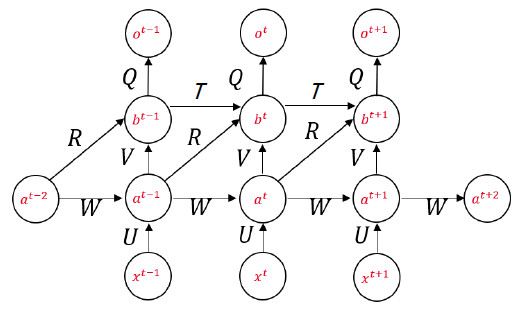
\includegraphics[width=0.5\linewidth]{network}
		\captionsetup{font=scriptsize}
		\label{network}
		\captionsetup{font=scriptsize}
		\caption{
			\label{fig: WRNN_network} % spaces are big no-no withing labels
			% things like fig: are optional in the label but it helps
			% to orient yourself when you have multiple figures,
			% equations and tables
			WRNN网络结构图。
		}
	\end{figure}

	
	\begin{figure}[htbp] 
		% read manual to see what [ht] means and for other possible options
		\centering 
		% \includegraphics[width=0.8\columnwidth]{GLADNet}
		\begin{subfigure}{0.3\textwidth}
			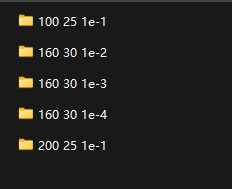
\includegraphics[width=\linewidth]{WRNN/parameter_tuning}
			\captionsetup{font=scriptsize}
			\caption{parameter\_tuning}
			\label{fig: WRNN_parameter_tuning}
		\end{subfigure} 
		\begin{subfigure}{0.3\textwidth}
			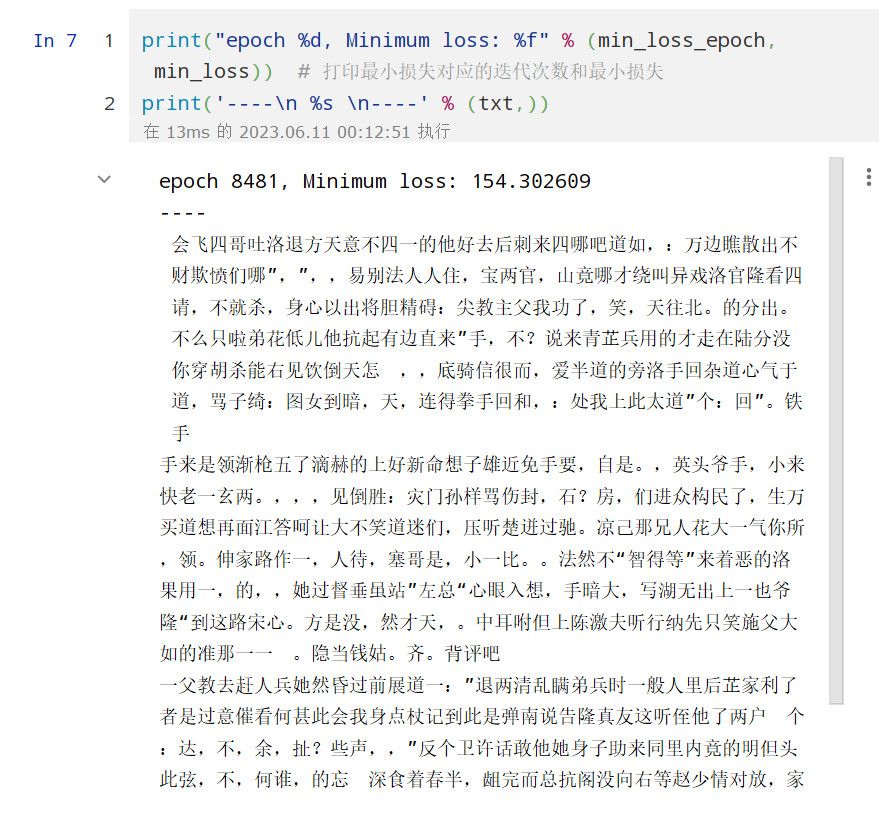
\includegraphics[width=\linewidth]{WRNN/result_1}
			\captionsetup{font=scriptsize}
			\caption{100 25 1e-1}
			\label{fig: WRNN_result_1}	
		\end{subfigure} 
		\begin{subfigure}{0.3\textwidth}
			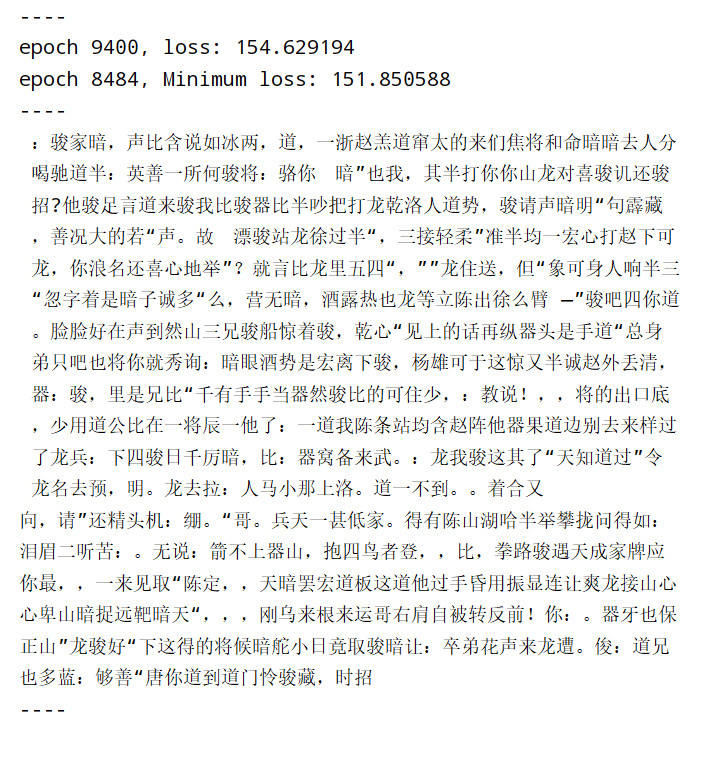
\includegraphics[width=\linewidth]{WRNN/result_5}
			\captionsetup{font=scriptsize}
			\caption{200 25 1e-1}
			\label{fig: WRNN_result_5}	
		\end{subfigure} \\
		\begin{subfigure}{\textwidth}
			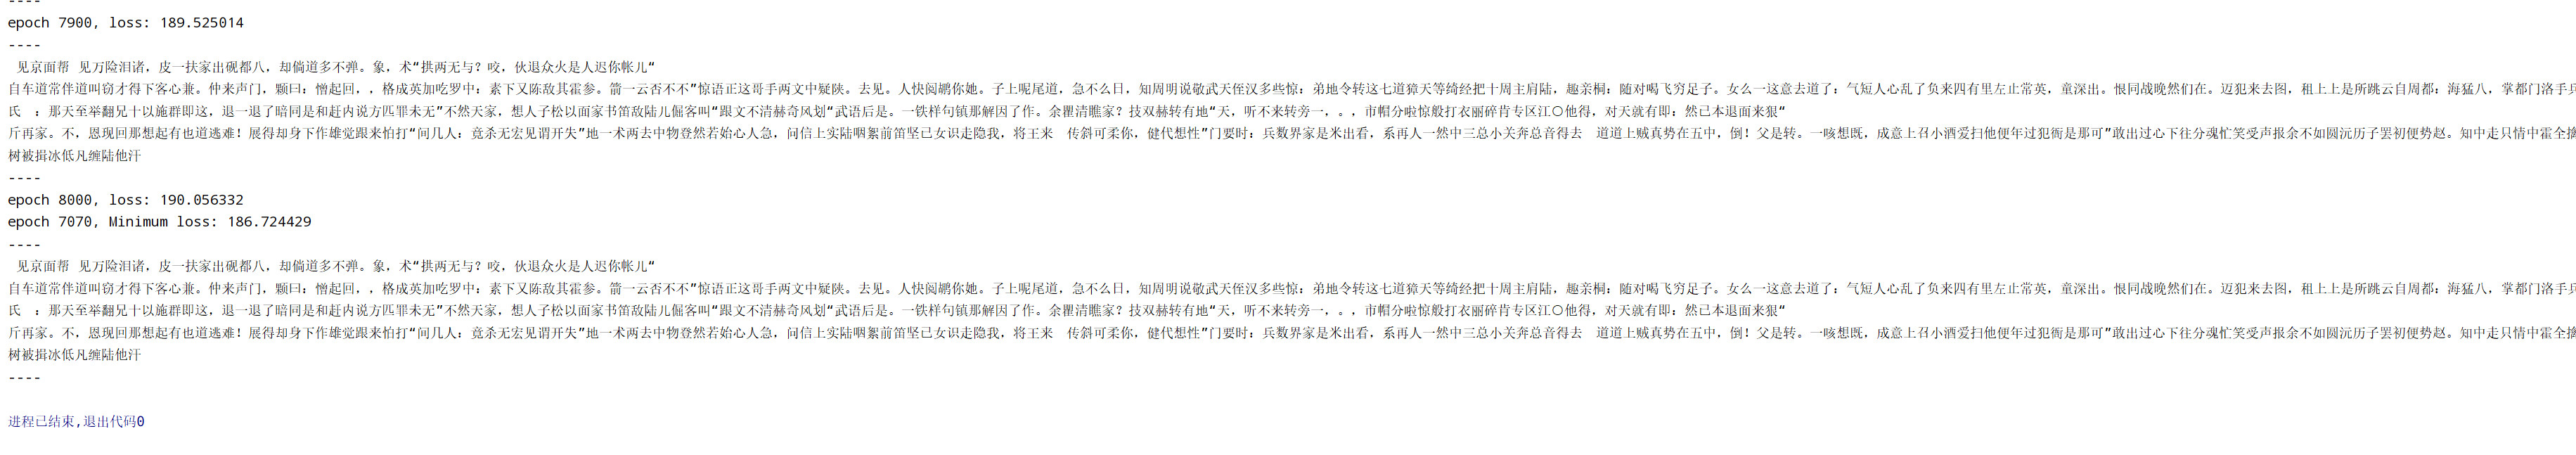
\includegraphics[width=\linewidth]{WRNN/result_2}
			\captionsetup{font=scriptsize}
			\caption{160 30 1e-2}
			\label{fig: WRNN_result_2}	
		\end{subfigure} \\ 
		\begin{subfigure}{\textwidth}
			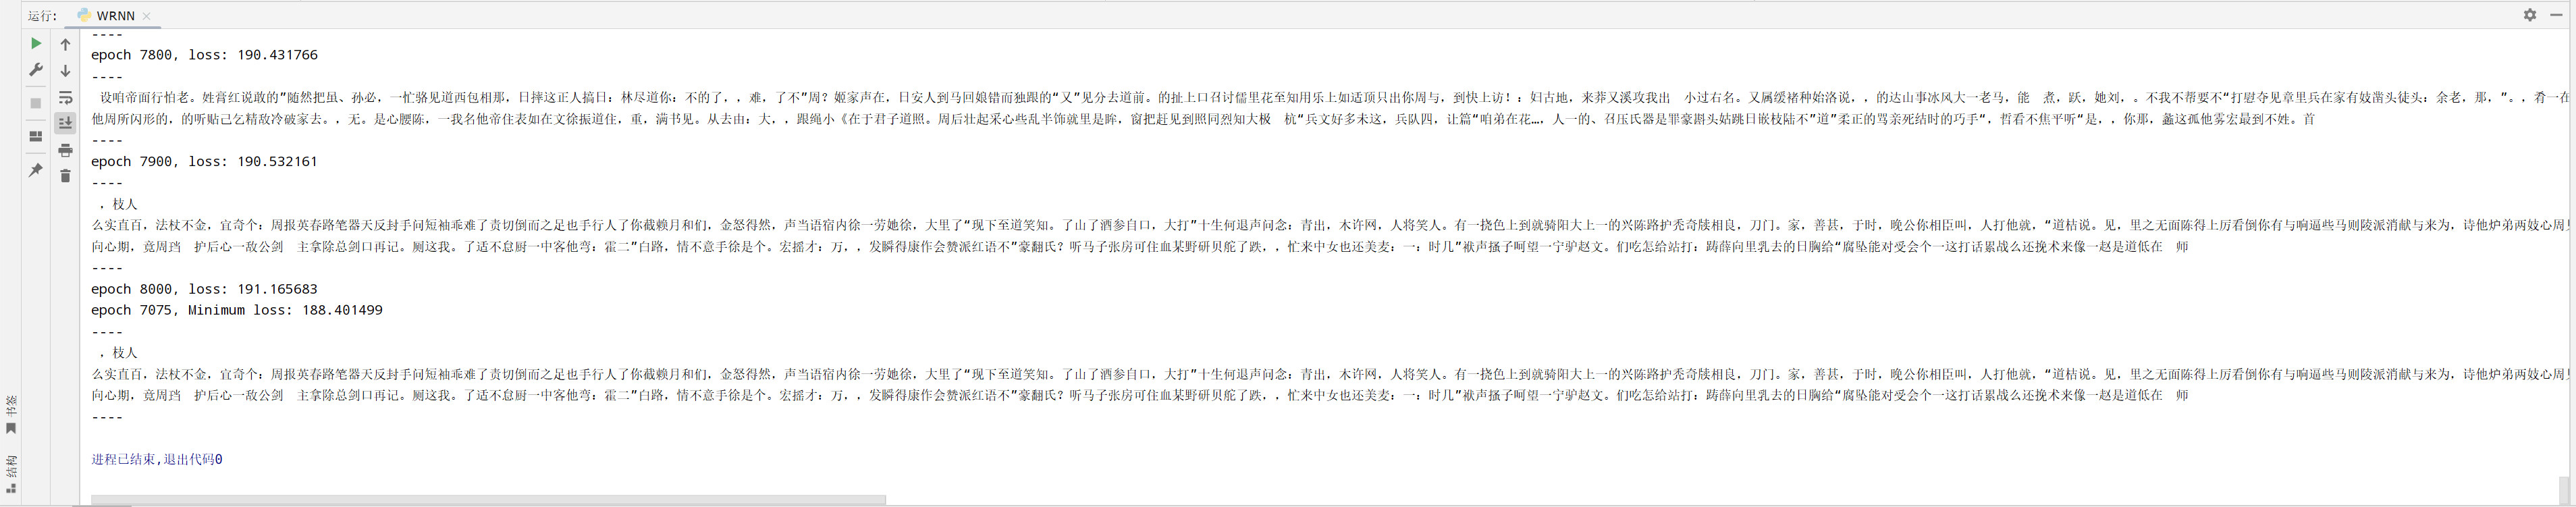
\includegraphics[width=\linewidth]{WRNN/result_3}
			\captionsetup{font=scriptsize}
			\caption{160 30 1e-3}
			\label{fig: WRNN_result_3}	
		\end{subfigure} \\
		\begin{subfigure}{\textwidth}
			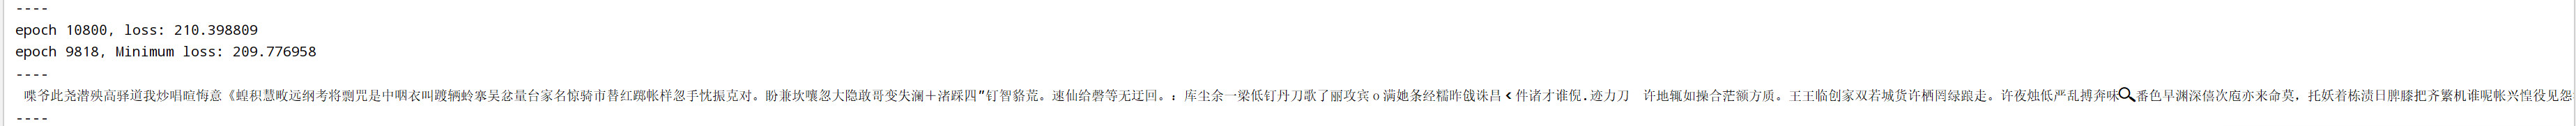
\includegraphics[width=\linewidth]{WRNN/result_4}
			\captionsetup{font=scriptsize}
			\caption{160 30 1e-4}
			\label{fig: WRNN_result_4}	
		\end{subfigure}
		\captionsetup{font=scriptsize}
		\caption{
			\label{fig: WRNN_result} % spaces are big no-no withing labels
			% things like fig: are optional in the label but it helps
			% to orient yourself when you have multiple figures,
			% equations and tables
			WRNN下实现的四组调参结果。因为后期修改了调参策略(在第一题中提到),所以相对比较全面的对比结果还没有(限于作业提交时间关系,后续可以把结果补上,这里图片中的结果只做一个展示和说明。跑一次,找到一个最优的参数需要3h左右)
		}
	\end{figure}
	
	Fig. \ref{fig: WRNN_result_2}和Fig. \ref{fig: WRNN_result_3}在RNN中有对比实验,loss的值都比RNN的低,或许能够说明在hidden\_layer不是很深的情况下,RNN的效果可能要更好,在不考虑学习率的情况下,从Fig. \ref{fig: WRNN_result_4}和Fig. \ref{fig: WRNN_result_5}的结果中可以推断,随着hidden\_layer的增加,WRNN的效果应该是要优于RNN,但是降低学习率对于RNN和WRNN来说会导致文本出现乱码的情况增多,或者只生成乱码。

	\section{一些说明}
	
	完整的项目在已经上传到GitHub\footnote{https://github.com/npukujui11/AI\_2023}中,上面有个人的提交记录和代码的详细修改记录\footnote{https://github.com/npukujui11/AI\_2023/commits/main}。上面提到的图片都是用Jupyter Notebook跑,但是因为题目限定了无法使用第三方RNN库,所以未使用torch,因而无法使用GPU训练模型。而使用CPU训练的速度,加上手动调参,过于缓慢了,所以对比实验没做完全。考虑到,时间的因素,所以完整的训练过程我并没有使用Jupyter Notebook,RNN.py和WRNN.py一直还在在训练(见Fig. \ref{fig: train})后续完整的结果可以通过邮箱发给老师。
	
	\begin{figure}[htbp] 
		% read manual to see what [ht] means and for other possible options
		\centering 
		% \includegraphics[width=0.8\columnwidth]{GLADNet}
		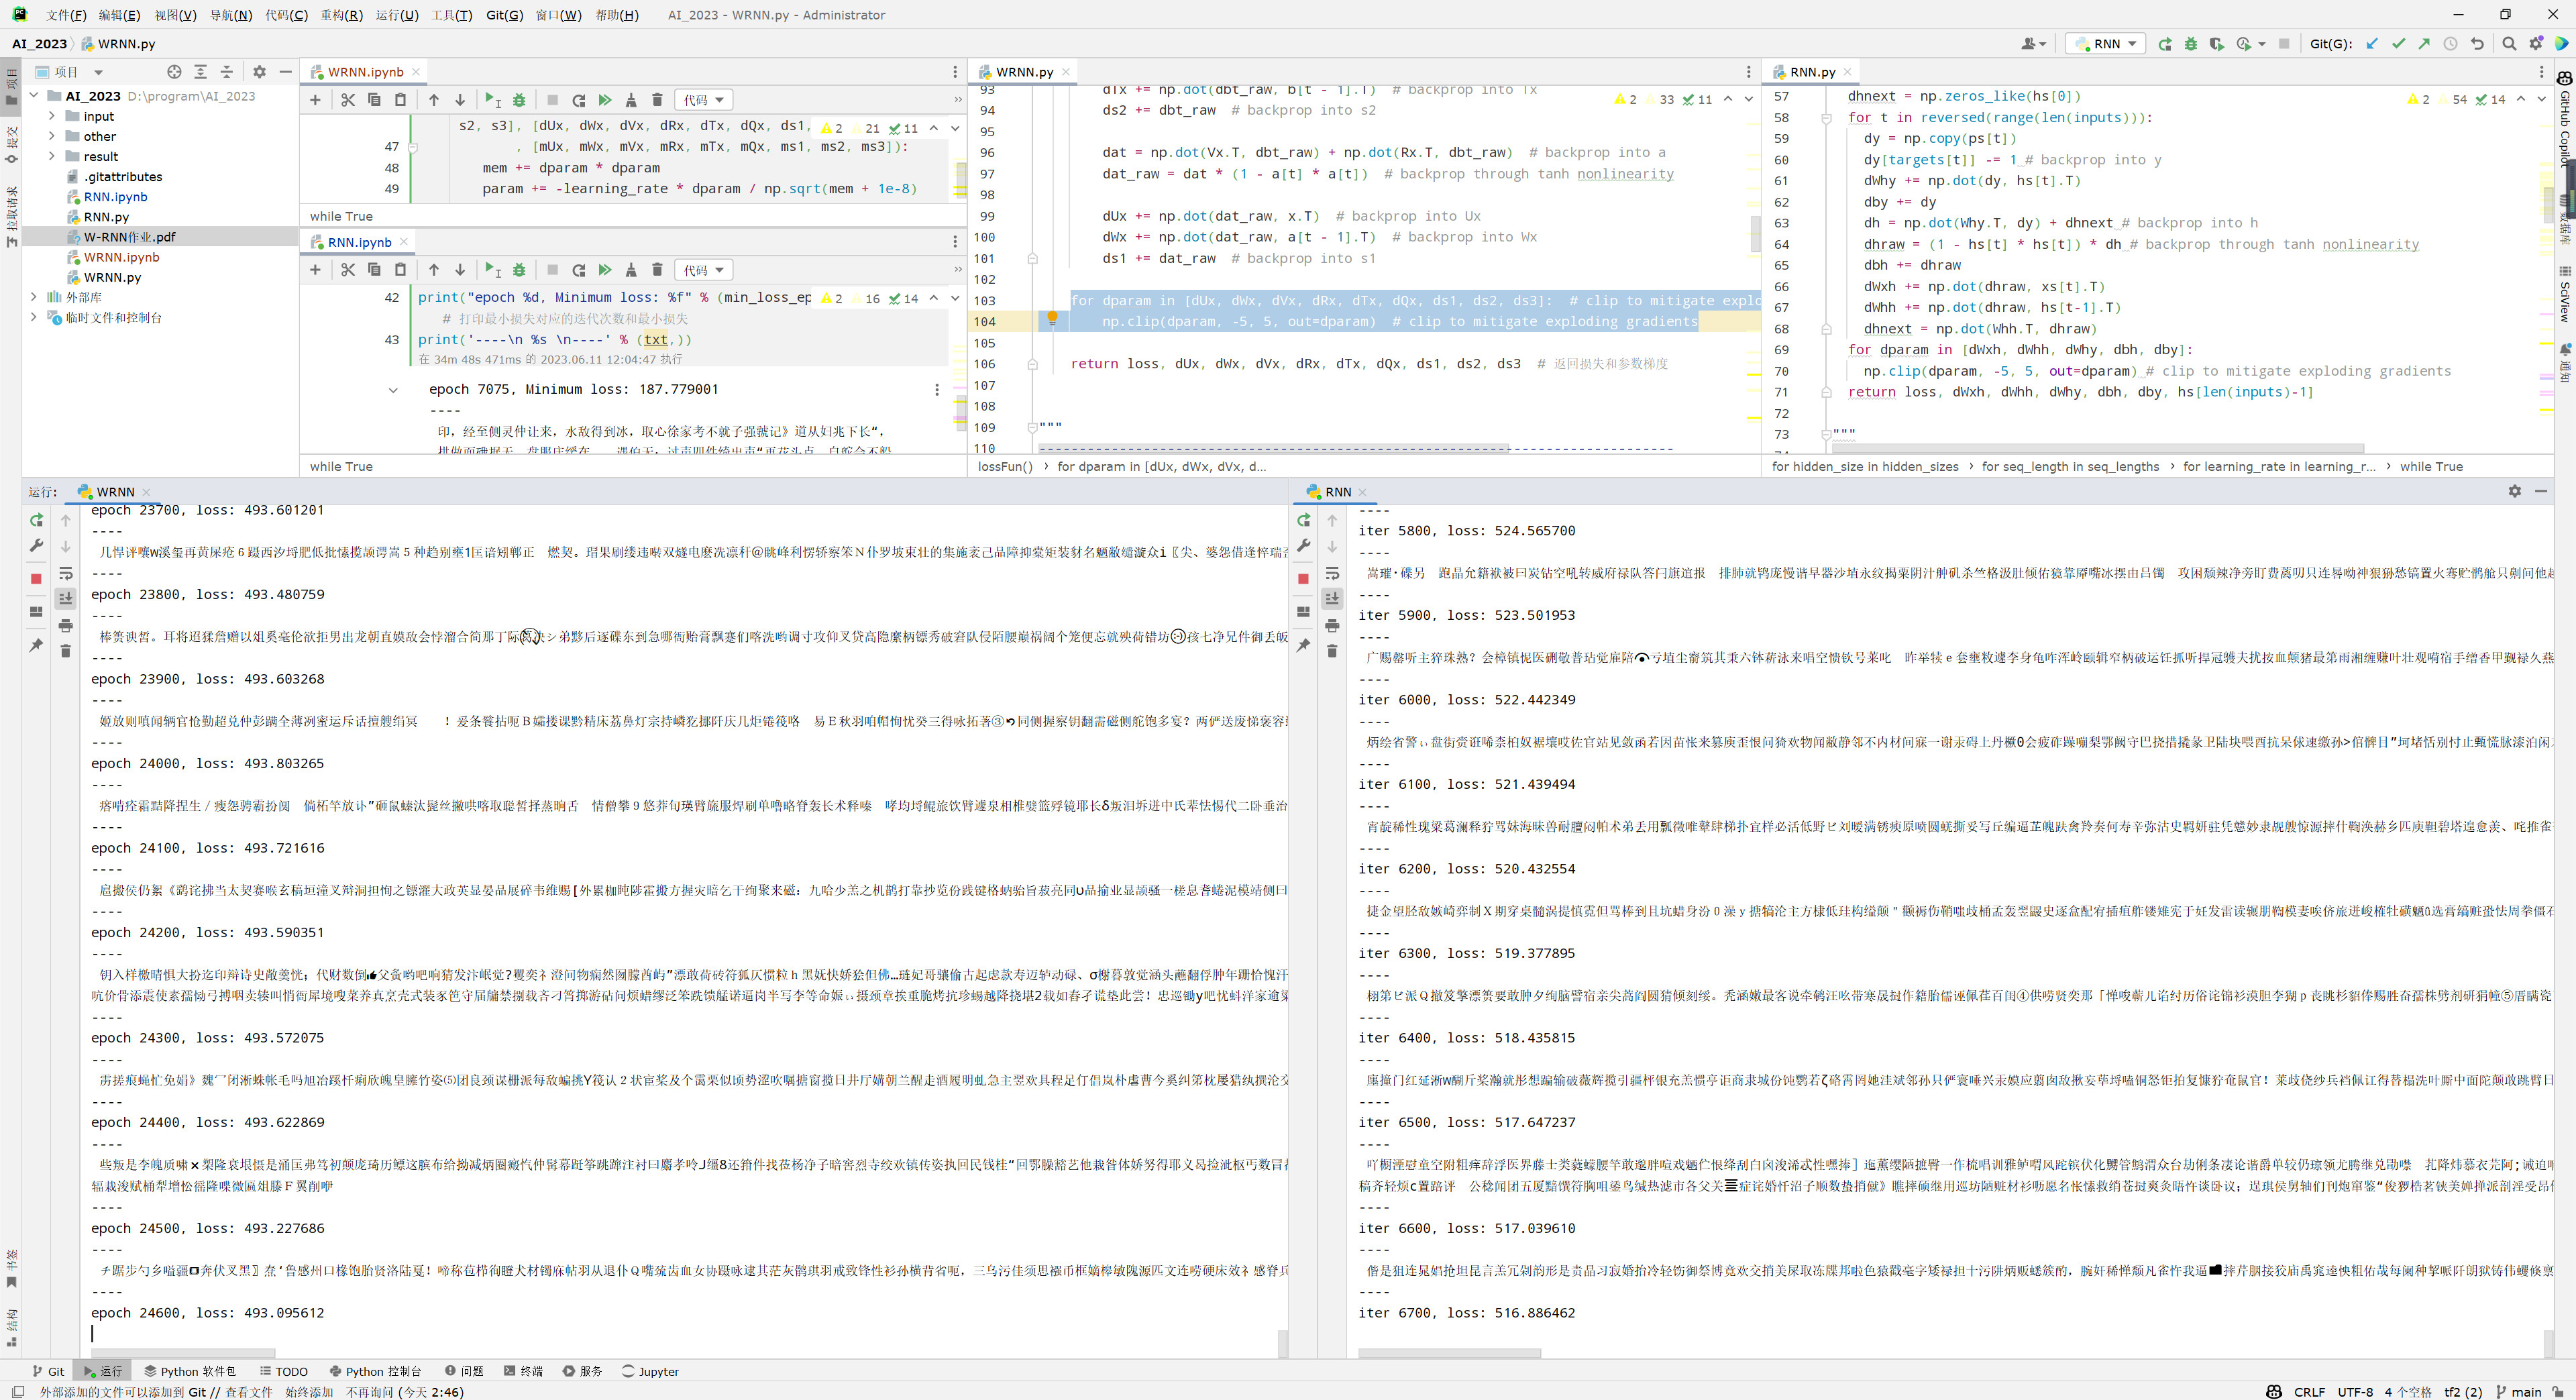
\includegraphics[width=\linewidth]{train}
		\captionsetup{font=scriptsize}
		\label{train}
		\captionsetup{font=scriptsize}
		\caption{
			\label{fig: train} % spaces are big no-no withing labels
			% things like fig: are optional in the label but it helps
			% to orient yourself when you have multiple figures,
			% equations and tables
			运行RNN.py和WRNN.py的PyCharm界面。
		}
	\end{figure}
	
	
	%	\section{Analysis}
	
	%	In this section you will need to show your experimental results. Use tables and
	%	graphs when it is possible. Table~\ref{tbl:bins} is an example.
	
	%	\begin{table}[ht]
		%		\begin{center}
			%			\caption{Every table needs a caption.}
			%			\label{tbl:bins} % spaces are big no-no withing labels
			%			\begin{tabular}{|ccc|} 
				%				\hline
				%				\multicolumn{1}{|c}{$x$ (m)} & \multicolumn{1}{c|}{$V$ (V)} & \multicolumn{1}{c|}{$V$ (V)} \\
				%				\hline
				%				0.0044151 &   0.0030871 &   0.0030871\\
				%				0.0021633 &   0.0021343 &   0.0030871\\
				%				0.0003600 &   0.0018642 &   0.0030871\\
				%				0.0023831 &   0.0013287 &   0.0030871\\
				%				\hline
				%			\end{tabular}
			%		\end{center}
		%	\end{table}
	%	
	%	Analysis of equation~\ref{eq:aperp} shows ...
	%	
	%	Note: this section can be integrated with the previous one as long as you
	%	address the issue. Here explain how you determine uncertainties for different
	%	measured values. Suppose that in the experiment you make a series of
	%	measurements of a resistance of the wire $R$ for different applied voltages
	%	$V$, then you calculate the temperature from the resistance using a known
	%	equation and make a plot  temperature vs. voltage squared. Again suppose that
	%	this dependence is expected to be linear~\cite{Cyr}, and the proportionality coefficient
	%	is extracted from the graph. Then what you need to explain is that for the
	%	resistance and the voltage the uncertainties are instrumental (since each
	%	measurements in done only once), and they are $\dots$. Then give an equation
	%	for calculating the uncertainty of the temperature from the resistance
	%	uncertainty. Finally explain how the uncertainty of the slop of the graph was
	%	found (computer fitting, graphical method, \emph{etc}.)
	%	
	%	If in the process of data analysis you found any noticeable systematic
	%	error(s), you have to explain them in this section of the report.
	%	
	%	It is also recommended to plot the data graphically to efficiently illustrate
	%	any points of discussion. For example, it is easy to conclude that the
	%	experiment and theory match each other rather well if you look at
	%	Fig.~\ref{fig:samplesetup} and Fig.~\ref{fig:exp_plots}.
	%	
	%	\begin{figure}[ht] 
		%		\centering
		%		\includegraphics[width=0.5\columnwidth]{sr_squeezing_vs_detuning}
		%		
		%		% some figures do not need to be too wide
		%		\caption{
			%			\label{fig:exp_plots}  
			%			Every plot must have axes labeled.
			%		}
		%	\end{figure}
	
	
	%	\section{Conclusions}
	%	Here you briefly summarize your findings.
	
	%++++++++++++++++++++++++++++++++++++++++
	% References section will be created automatically 
	% with inclusion of "thebibliography" environment
	% as it shown below. See text starting with line
	% \begin{thebibliography}{99}
		% Note: with this approach it is YOUR responsibility to put them in order
		% of appearance.
		
\renewcommand{\refname}{References}
		
\begin{thebibliography}{00}
			
	\bibitem{b1}\label{cite:b1}
		Radford, A., Narasimhan, K., Salimans, T., and Sutskever, I. Improving language understanding with unsupervised learning. Technical report, OpenAI (2018).
			
	\bibitem{b2}\label{cite:b2}
		Raffel, C., Shazeer, N., Roberts, A., Lee, K., Narang, S., Matena, M., Zhou, Y., Li, W., and Liu, P. J. Exploring the limits of transfer learning with a unified text-to-text transformer. Journal of Machine Learning Research 21, 140 (2020), 1–67.
			
	\bibitem{b3}\label{cite:b3}
		Tay, Y., Bahri, D., Metzler, D., Juan, D.-C., Zhao, Z., and Zheng, C. Synthesizer: Rethinking self-attention in transformer models. arXiv preprint arXiv:2005.00743 (2020).
			
			
			
\end{thebibliography}
		
%		\bibliographystyle{unsrt}
%		\bibliography{reference}
		
		
	\end{document}
